\documentclass[10pt,a4paper]{article}
\usepackage{ucs}
\usepackage[a4paper,top=2cm,bottom=2cm,left=3cm,right=3cm,marginparwidth=1.75cm]{geometry}

\usepackage[utf8x]{inputenc}
\usepackage[hebrew, english]{babel}
% \usepackage{culmus}
%%%%% NEW MATH DEFINITIONS %%%%%

\usepackage{amsmath,amsfonts,bm}

% Mark sections of captions for referring to divisions of figures
\newcommand{\figleft}{{\em (Left)}}
\newcommand{\figcenter}{{\em (Center)}}
\newcommand{\figright}{{\em (Right)}}
\newcommand{\figtop}{{\em (Top)}}
\newcommand{\figbottom}{{\em (Bottom)}}
\newcommand{\captiona}{{\em (a)}}
\newcommand{\captionb}{{\em (b)}}
\newcommand{\captionc}{{\em (c)}}
\newcommand{\captiond}{{\em (d)}}

% Highlight a newly defined term
\newcommand{\newterm}[1]{{\bf #1}}


% Figure reference, lower-case.
\def\figref#1{figure~\ref{#1}}
% Figure reference, capital. For start of sentence
\def\Figref#1{Figure~\ref{#1}}
\def\twofigref#1#2{figures \ref{#1} and \ref{#2}}
\def\quadfigref#1#2#3#4{figures \ref{#1}, \ref{#2}, \ref{#3} and \ref{#4}}
% Section reference, lower-case.
\def\secref#1{section~\ref{#1}}
% Section reference, capital.
\def\Secref#1{Section~\ref{#1}}
% Reference to two sections.
\def\twosecrefs#1#2{sections \ref{#1} and \ref{#2}}
% Reference to three sections.
\def\secrefs#1#2#3{sections \ref{#1}, \ref{#2} and \ref{#3}}
% Reference to an equation, lower-case.
\def\eqref#1{equation~\ref{#1}}
% Reference to an equation, upper case
\def\Eqref#1{Equation~\ref{#1}}
% A raw reference to an equation---avoid using if possible
\def\plaineqref#1{\ref{#1}}
% Reference to a chapter, lower-case.
\def\chapref#1{chapter~\ref{#1}}
% Reference to an equation, upper case.
\def\Chapref#1{Chapter~\ref{#1}}
% Reference to a range of chapters
\def\rangechapref#1#2{chapters\ref{#1}--\ref{#2}}
% Reference to an algorithm, lower-case.
\def\algref#1{algorithm~\ref{#1}}
% Reference to an algorithm, upper case.
\def\Algref#1{Algorithm~\ref{#1}}
\def\twoalgref#1#2{algorithms \ref{#1} and \ref{#2}}
\def\Twoalgref#1#2{Algorithms \ref{#1} and \ref{#2}}
% Reference to a part, lower case
\def\partref#1{part~\ref{#1}}
% Reference to a part, upper case
\def\Partref#1{Part~\ref{#1}}
\def\twopartref#1#2{parts \ref{#1} and \ref{#2}}

\def\ceil#1{\lceil #1 \rceil}
\def\floor#1{\lfloor #1 \rfloor}
\def\1{\bm{1}}
\newcommand{\train}{\mathcal{D}}
\newcommand{\valid}{\mathcal{D_{\mathrm{valid}}}}
\newcommand{\test}{\mathcal{D_{\mathrm{test}}}}

\def\eps{{\epsilon}}


% Random variables
\def\reta{{\textnormal{$\eta$}}}
\def\ra{{\textnormal{a}}}
\def\rb{{\textnormal{b}}}
\def\rc{{\textnormal{c}}}
\def\rd{{\textnormal{d}}}
\def\re{{\textnormal{e}}}
\def\rf{{\textnormal{f}}}
\def\rg{{\textnormal{g}}}
\def\rh{{\textnormal{h}}}
\def\ri{{\textnormal{i}}}
\def\rj{{\textnormal{j}}}
\def\rk{{\textnormal{k}}}
\def\rl{{\textnormal{l}}}
% rm is already a command, just don't name any random variables m
\def\rn{{\textnormal{n}}}
\def\ro{{\textnormal{o}}}
\def\rp{{\textnormal{p}}}
\def\rq{{\textnormal{q}}}
\def\rr{{\textnormal{r}}}
\def\rs{{\textnormal{s}}}
\def\rt{{\textnormal{t}}}
\def\ru{{\textnormal{u}}}
\def\rv{{\textnormal{v}}}
\def\rw{{\textnormal{w}}}
\def\rx{{\textnormal{x}}}
\def\ry{{\textnormal{y}}}
\def\rz{{\textnormal{z}}}

% Random vectors
\def\rvepsilon{{\mathbf{\epsilon}}}
\def\rvtheta{{\mathbf{\theta}}}
\def\rva{{\mathbf{a}}}
\def\rvb{{\mathbf{b}}}
\def\rvc{{\mathbf{c}}}
\def\rvd{{\mathbf{d}}}
\def\rve{{\mathbf{e}}}
\def\rvf{{\mathbf{f}}}
\def\rvg{{\mathbf{g}}}
\def\rvh{{\mathbf{h}}}
\def\rvu{{\mathbf{i}}}
\def\rvj{{\mathbf{j}}}
\def\rvk{{\mathbf{k}}}
\def\rvl{{\mathbf{l}}}
\def\rvm{{\mathbf{m}}}
\def\rvn{{\mathbf{n}}}
\def\rvo{{\mathbf{o}}}
\def\rvp{{\mathbf{p}}}
\def\rvq{{\mathbf{q}}}
\def\rvr{{\mathbf{r}}}
\def\rvs{{\mathbf{s}}}
\def\rvt{{\mathbf{t}}}
\def\rvu{{\mathbf{u}}}
\def\rvv{{\mathbf{v}}}
\def\rvw{{\mathbf{w}}}
\def\rvx{{\mathbf{x}}}
\def\rvy{{\mathbf{y}}}
\def\rvz{{\mathbf{z}}}

% Elements of random vectors
\def\erva{{\textnormal{a}}}
\def\ervb{{\textnormal{b}}}
\def\ervc{{\textnormal{c}}}
\def\ervd{{\textnormal{d}}}
\def\erve{{\textnormal{e}}}
\def\ervf{{\textnormal{f}}}
\def\ervg{{\textnormal{g}}}
\def\ervh{{\textnormal{h}}}
\def\ervi{{\textnormal{i}}}
\def\ervj{{\textnormal{j}}}
\def\ervk{{\textnormal{k}}}
\def\ervl{{\textnormal{l}}}
\def\ervm{{\textnormal{m}}}
\def\ervn{{\textnormal{n}}}
\def\ervo{{\textnormal{o}}}
\def\ervp{{\textnormal{p}}}
\def\ervq{{\textnormal{q}}}
\def\ervr{{\textnormal{r}}}
\def\ervs{{\textnormal{s}}}
\def\ervt{{\textnormal{t}}}
\def\ervu{{\textnormal{u}}}
\def\ervv{{\textnormal{v}}}
\def\ervw{{\textnormal{w}}}
\def\ervx{{\textnormal{x}}}
\def\ervy{{\textnormal{y}}}
\def\ervz{{\textnormal{z}}}

% Random matrices
\def\rmA{{\mathbf{A}}}
\def\rmB{{\mathbf{B}}}
\def\rmC{{\mathbf{C}}}
\def\rmD{{\mathbf{D}}}
\def\rmE{{\mathbf{E}}}
\def\rmF{{\mathbf{F}}}
\def\rmG{{\mathbf{G}}}
\def\rmH{{\mathbf{H}}}
\def\rmI{{\mathbf{I}}}
\def\rmJ{{\mathbf{J}}}
\def\rmK{{\mathbf{K}}}
\def\rmL{{\mathbf{L}}}
\def\rmM{{\mathbf{M}}}
\def\rmN{{\mathbf{N}}}
\def\rmO{{\mathbf{O}}}
\def\rmP{{\mathbf{P}}}
\def\rmQ{{\mathbf{Q}}}
\def\rmR{{\mathbf{R}}}
\def\rmS{{\mathbf{S}}}
\def\rmT{{\mathbf{T}}}
\def\rmU{{\mathbf{U}}}
\def\rmV{{\mathbf{V}}}
\def\rmW{{\mathbf{W}}}
\def\rmX{{\mathbf{X}}}
\def\rmY{{\mathbf{Y}}}
\def\rmZ{{\mathbf{Z}}}

% Elements of random matrices
\def\ermA{{\textnormal{A}}}
\def\ermB{{\textnormal{B}}}
\def\ermC{{\textnormal{C}}}
\def\ermD{{\textnormal{D}}}
\def\ermE{{\textnormal{E}}}
\def\ermF{{\textnormal{F}}}
\def\ermG{{\textnormal{G}}}
\def\ermH{{\textnormal{H}}}
\def\ermI{{\textnormal{I}}}
\def\ermJ{{\textnormal{J}}}
\def\ermK{{\textnormal{K}}}
\def\ermL{{\textnormal{L}}}
\def\ermM{{\textnormal{M}}}
\def\ermN{{\textnormal{N}}}
\def\ermO{{\textnormal{O}}}
\def\ermP{{\textnormal{P}}}
\def\ermQ{{\textnormal{Q}}}
\def\ermR{{\textnormal{R}}}
\def\ermS{{\textnormal{S}}}
\def\ermT{{\textnormal{T}}}
\def\ermU{{\textnormal{U}}}
\def\ermV{{\textnormal{V}}}
\def\ermW{{\textnormal{W}}}
\def\ermX{{\textnormal{X}}}
\def\ermY{{\textnormal{Y}}}
\def\ermZ{{\textnormal{Z}}}

% Vectors
\def\vzero{{\bm{0}}}
\def\vone{{\bm{1}}}
\def\vmu{{\bm{\mu}}}
\def\vtheta{{\bm{\theta}}}
\def\va{{\bm{a}}}
\def\vb{{\bm{b}}}
\def\vc{{\bm{c}}}
\def\vd{{\bm{d}}}
\def\ve{{\bm{e}}}
\def\vf{{\bm{f}}}
\def\vg{{\bm{g}}}
\def\vh{{\bm{h}}}
\def\vi{{\bm{i}}}
\def\vj{{\bm{j}}}
\def\vk{{\bm{k}}}
\def\vl{{\bm{l}}}
\def\vm{{\bm{m}}}
\def\vn{{\bm{n}}}
\def\vo{{\bm{o}}}
\def\vp{{\bm{p}}}
\def\vq{{\bm{q}}}
\def\vr{{\bm{r}}}
\def\vs{{\bm{s}}}
\def\vt{{\bm{t}}}
\def\vu{{\bm{u}}}
\def\vv{{\bm{v}}}
\def\vw{{\bm{w}}}
\def\vx{{\bm{x}}}
\def\vy{{\bm{y}}}
\def\vz{{\bm{z}}}

% Elements of vectors
\def\evalpha{{\alpha}}
\def\evbeta{{\beta}}
\def\evepsilon{{\epsilon}}
\def\evlambda{{\lambda}}
\def\evomega{{\omega}}
\def\evmu{{\mu}}
\def\evpsi{{\psi}}
\def\evsigma{{\sigma}}
\def\evtheta{{\theta}}
\def\eva{{a}}
\def\evb{{b}}
\def\evc{{c}}
\def\evd{{d}}
\def\eve{{e}}
\def\evf{{f}}
\def\evg{{g}}
\def\evh{{h}}
\def\evi{{i}}
\def\evj{{j}}
\def\evk{{k}}
\def\evl{{l}}
\def\evm{{m}}
\def\evn{{n}}
\def\evo{{o}}
\def\evp{{p}}
\def\evq{{q}}
\def\evr{{r}}
\def\evs{{s}}
\def\evt{{t}}
\def\evu{{u}}
\def\evv{{v}}
\def\evw{{w}}
\def\evx{{x}}
\def\evy{{y}}
\def\evz{{z}}

% Matrix
\def\mA{{\bm{A}}}
\def\mB{{\bm{B}}}
\def\mC{{\bm{C}}}
\def\mD{{\bm{D}}}
\def\mE{{\bm{E}}}
\def\mF{{\bm{F}}}
\def\mG{{\bm{G}}}
\def\mH{{\bm{H}}}
\def\mI{{\bm{I}}}
\def\mJ{{\bm{J}}}
\def\mK{{\bm{K}}}
\def\mL{{\bm{L}}}
\def\mM{{\bm{M}}}
\def\mN{{\bm{N}}}
\def\mO{{\bm{O}}}
\def\mP{{\bm{P}}}
\def\mQ{{\bm{Q}}}
\def\mR{{\bm{R}}}
\def\mS{{\bm{S}}}
\def\mT{{\bm{T}}}
\def\mU{{\bm{U}}}
\def\mV{{\bm{V}}}
\def\mW{{\bm{W}}}
\def\mX{{\bm{X}}}
\def\mY{{\bm{Y}}}
\def\mZ{{\bm{Z}}}
\def\mBeta{{\bm{\beta}}}
\def\mPhi{{\bm{\Phi}}}
\def\mLambda{{\bm{\Lambda}}}
\def\mSigma{{\bm{\Sigma}}}

% Tensor
\DeclareMathAlphabet{\mathsfit}{\encodingdefault}{\sfdefault}{m}{sl}
\SetMathAlphabet{\mathsfit}{bold}{\encodingdefault}{\sfdefault}{bx}{n}
\newcommand{\tens}[1]{\bm{\mathsfit{#1}}}
\def\tA{{\tens{A}}}
\def\tB{{\tens{B}}}
\def\tC{{\tens{C}}}
\def\tD{{\tens{D}}}
\def\tE{{\tens{E}}}
\def\tF{{\tens{F}}}
\def\tG{{\tens{G}}}
\def\tH{{\tens{H}}}
\def\tI{{\tens{I}}}
\def\tJ{{\tens{J}}}
\def\tK{{\tens{K}}}
\def\tL{{\tens{L}}}
\def\tM{{\tens{M}}}
\def\tN{{\tens{N}}}
\def\tO{{\tens{O}}}
\def\tP{{\tens{P}}}
\def\tQ{{\tens{Q}}}
\def\tR{{\tens{R}}}
\def\tS{{\tens{S}}}
\def\tT{{\tens{T}}}
\def\tU{{\tens{U}}}
\def\tV{{\tens{V}}}
\def\tW{{\tens{W}}}
\def\tX{{\tens{X}}}
\def\tY{{\tens{Y}}}
\def\tZ{{\tens{Z}}}


% Graph
\def\gA{{\mathcal{A}}}
\def\gB{{\mathcal{B}}}
\def\gC{{\mathcal{C}}}
\def\gD{{\mathcal{D}}}
\def\gE{{\mathcal{E}}}
\def\gF{{\mathcal{F}}}
\def\gG{{\mathcal{G}}}
\def\gH{{\mathcal{H}}}
\def\gI{{\mathcal{I}}}
\def\gJ{{\mathcal{J}}}
\def\gK{{\mathcal{K}}}
\def\gL{{\mathcal{L}}}
\def\gM{{\mathcal{M}}}
\def\gN{{\mathcal{N}}}
\def\gO{{\mathcal{O}}}
\def\gP{{\mathcal{P}}}
\def\gQ{{\mathcal{Q}}}
\def\gR{{\mathcal{R}}}
\def\gS{{\mathcal{S}}}
\def\gT{{\mathcal{T}}}
\def\gU{{\mathcal{U}}}
\def\gV{{\mathcal{V}}}
\def\gW{{\mathcal{W}}}
\def\gX{{\mathcal{X}}}
\def\gY{{\mathcal{Y}}}
\def\gZ{{\mathcal{Z}}}

% Sets
\def\sA{{\mathbb{A}}}
\def\sB{{\mathbb{B}}}
\def\sC{{\mathbb{C}}}
\def\sD{{\mathbb{D}}}
% Don't use a set called E, because this would be the same as our symbol
% for expectation.
\def\sF{{\mathbb{F}}}
\def\sG{{\mathbb{G}}}
\def\sH{{\mathbb{H}}}
\def\sI{{\mathbb{I}}}
\def\sJ{{\mathbb{J}}}
\def\sK{{\mathbb{K}}}
\def\sL{{\mathbb{L}}}
\def\sM{{\mathbb{M}}}
\def\sN{{\mathbb{N}}}
\def\sO{{\mathbb{O}}}
\def\sP{{\mathbb{P}}}
\def\sQ{{\mathbb{Q}}}
\def\sR{{\mathbb{R}}}
\def\sS{{\mathbb{S}}}
\def\sT{{\mathbb{T}}}
\def\sU{{\mathbb{U}}}
\def\sV{{\mathbb{V}}}
\def\sW{{\mathbb{W}}}
\def\sX{{\mathbb{X}}}
\def\sY{{\mathbb{Y}}}
\def\sZ{{\mathbb{Z}}}

% Entries of a matrix
\def\emLambda{{\Lambda}}
\def\emA{{A}}
\def\emB{{B}}
\def\emC{{C}}
\def\emD{{D}}
\def\emE{{E}}
\def\emF{{F}}
\def\emG{{G}}
\def\emH{{H}}
\def\emI{{I}}
\def\emJ{{J}}
\def\emK{{K}}
\def\emL{{L}}
\def\emM{{M}}
\def\emN{{N}}
\def\emO{{O}}
\def\emP{{P}}
\def\emQ{{Q}}
\def\emR{{R}}
\def\emS{{S}}
\def\emT{{T}}
\def\emU{{U}}
\def\emV{{V}}
\def\emW{{W}}
\def\emX{{X}}
\def\emY{{Y}}
\def\emZ{{Z}}
\def\emSigma{{\Sigma}}

% entries of a tensor
% Same font as tensor, without \bm wrapper
\newcommand{\etens}[1]{\mathsfit{#1}}
\def\etLambda{{\etens{\Lambda}}}
\def\etA{{\etens{A}}}
\def\etB{{\etens{B}}}
\def\etC{{\etens{C}}}
\def\etD{{\etens{D}}}
\def\etE{{\etens{E}}}
\def\etF{{\etens{F}}}
\def\etG{{\etens{G}}}
\def\etH{{\etens{H}}}
\def\etI{{\etens{I}}}
\def\etJ{{\etens{J}}}
\def\etK{{\etens{K}}}
\def\etL{{\etens{L}}}
\def\etM{{\etens{M}}}
\def\etN{{\etens{N}}}
\def\etO{{\etens{O}}}
\def\etP{{\etens{P}}}
\def\etQ{{\etens{Q}}}
\def\etR{{\etens{R}}}
\def\etS{{\etens{S}}}
\def\etT{{\etens{T}}}
\def\etU{{\etens{U}}}
\def\etV{{\etens{V}}}
\def\etW{{\etens{W}}}
\def\etX{{\etens{X}}}
\def\etY{{\etens{Y}}}
\def\etZ{{\etens{Z}}}

% The true underlying data generating distribution
\newcommand{\pdata}{p_{\rm{data}}}
% The empirical distribution defined by the training set
\newcommand{\ptrain}{\hat{p}_{\rm{data}}}
\newcommand{\Ptrain}{\hat{P}_{\rm{data}}}
% The model distribution
\newcommand{\pmodel}{p_{\rm{model}}}
\newcommand{\Pmodel}{P_{\rm{model}}}
\newcommand{\ptildemodel}{\tilde{p}_{\rm{model}}}
% Stochastic autoencoder distributions
\newcommand{\pencode}{p_{\rm{encoder}}}
\newcommand{\pdecode}{p_{\rm{decoder}}}
\newcommand{\precons}{p_{\rm{reconstruct}}}

\newcommand{\laplace}{\mathrm{Laplace}} % Laplace distribution

\newcommand{\E}{\mathbb{E}}
\newcommand{\Ls}{\mathcal{L}}
% \newcommand{\R}{\mathbb{R}}
\newcommand{\emp}{\tilde{p}}
\newcommand{\lr}{\alpha}
\newcommand{\reg}{\lambda}
\newcommand{\rect}{\mathrm{rectifier}}
\newcommand{\softmax}{\mathrm{softmax}}
\newcommand{\sigmoid}{\sigma}
\newcommand{\softplus}{\zeta}
\newcommand{\KL}{D_{\mathrm{KL}}}
\newcommand{\Var}{\mathrm{Var}}
\newcommand{\standarderror}{\mathrm{SE}}
\newcommand{\Cov}{\mathrm{Cov}}
% Wolfram Mathworld says $L^2$ is for function spaces and $\ell^2$ is for vectors
% But then they seem to use $L^2$ for vectors throughout the site, and so does
% wikipedia.
\newcommand{\normlzero}{L^0}
\newcommand{\normlone}{L^1}
\newcommand{\normltwo}{L^2}
\newcommand{\normlp}{L^p}
\newcommand{\normmax}{L^\infty}

\newcommand{\parents}{Pa} % See usage in notation.tex. Chosen to match Daphne's book.

\DeclareMathOperator*{\argmax}{arg\,max}
\DeclareMathOperator*{\argmin}{arg\,min}

\DeclareMathOperator{\sign}{sign}
\DeclareMathOperator{\Tr}{Tr}
\let\ab\allowbreak

\usepackage{hyperref}
\usepackage{amsfonts}
\usepackage{amsmath,amssymb}
\usepackage{url}
\usepackage{derivative}
\usepackage{graphicx}
\usepackage{wrapfig}

\usepackage{caption}
\usepackage{subcaption}
\usepackage{listings}


% \usepackage[margin=0.5in]{geometry}
\newcommand{\T}{\theta}


\title{\foreignlanguage{english}{Optimization - Final Project}}
\author{Mor Hale and Yona Coscas}

\begin{document}
\maketitle
\section{Introduction}

\section*{The Problem}

An Artificial Neural Networks (ANNs or NNs) is based on a collection of connected units or nodes called artificial neurons, which loosely model the neurons in a biological brain. An artificial neuron receives a signal then processes it and can signal neurons connected to it. Each connection, like the synapses in a biological brain, can transmit a signal to other neurons. The "signal" at a connection is a real number, and the output of each neuron is computed by some non-linear function of the sum of its inputs. Typically, neurons are aggregated into layers. Signals travel from the first layer (the input layer),through the hidden layers, to the last layer (the output layer).\\

\begin{center}
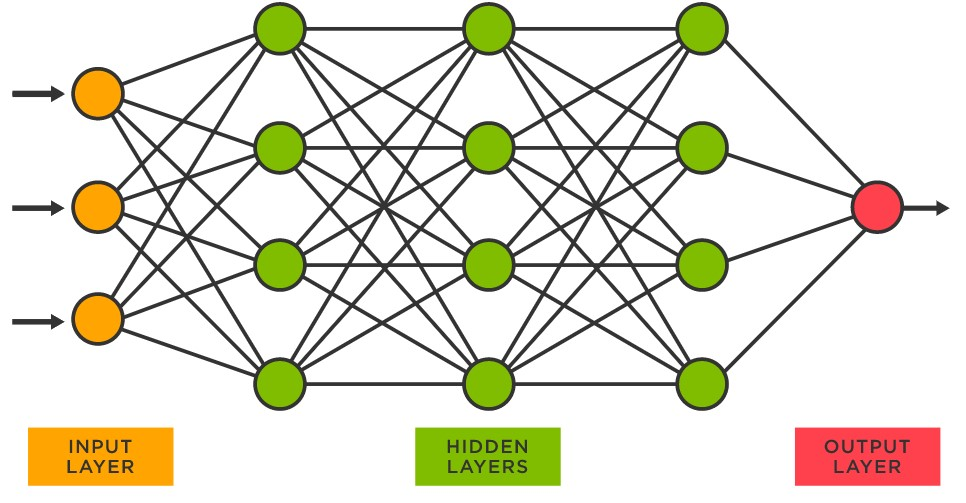
\includegraphics[width=10cm, height=5cm]{neutral-network-diagram.jpg}
\end{center}

In supervised learning, neural network learn (or are trained) by processing examples, each of which contains a known "input" and "result," forming probability-weighted associations between the two, which are stored within the data structure of the net itself. The training of a neural network from a given example is usually conducted by determining the difference between the processed output of the network (often a prediction) and a target output. This difference is the error or loss. The network then optimize its weighted associations according to a learning rule and using this error value. Successive adjustments will cause the neural network to produce output which is increasingly similar to the target output. After a sufficient number of these adjustments the training can be terminated based upon certain criteria.\\

The setting for a simple neural network optimization setup, is firstly a training dataset $D$, secondly a model $\hat{f}_{\theta}(x)$ with parameters $\theta$ that can be updated and lastly an loss function $L(\theta)$ that represents the accuracy of the model.
The goal of the optimization process is to find the parameters that minimize the loss function on the training set.\\





\section*{The Optimizer}

ADAM, stands for ADAptive Moment estimation, is an gradient based optimization algorithm for stochastic differentiable functions. In this algorithm we use only first order derivitives so it is better then second-order methods such as Newton's.
It is also a stochastic algorithm, i.e., it does not require calculating the gradients for the whole dataset. Instead it samples randomly from the dataset and optimize the parameters based on this sample, which reduce the computation time.
The stochastic approach has been the main solution for deep learning models.\\


[since it is a procedural optimization process that continues until convergence, we want to minimize the expected value of this function $\mathbf{E}[L_i(\theta)]$, with $L_1(\theta), ...L_T(\theta)$ being the realization of the function at subsequent timestamps 1,...,T.]\\ 


Let $g=\nabla_\theta L_t(\theta)$ be the vector of partial derivatives of $L_t(\theta)$, w.r.t $\theta$ evaluated at timestamp t. For the algorithm we will use: 
\begin{equation*}
    m_t=\beta_1m_{t-1}+(1-\beta_1)g_t
\end{equation*}
which is the exponential moving average of the first moment of the gradient (mean) weighted with the parameter $\beta_1\in[0,1)$ and: 
\begin{equation*}
    v_t=\beta_2v_{t-1}+(1-\beta_2)g^2_t
\end{equation*}
being the weighted average of the second moment of the gradient (the uncentered variance) with $\beta_2\in[0,1)$. $\beta_1$ and $\beta_2$ control the exponential decay rates of these moving averages, and set to be 0.9, 0.999 respectively according to the author [*****add reference*****].
Both $m_t$ and $v_t$ are vectors initialized to zeros, which make the moments estimates to be biased towards zeros especially when the $\beta$s become closer to 1, so we need to fix them to be bias corrected, the resulting estimates are: 
\begin{equation*}
    \begin{split}
    \hat{m}_t=\frac{m_t}{1-\beta_1^t} \\ 
    \hat{v}_t=\frac{v_t}{1-\beta_2^t}
    \end{split}
\end{equation*}

then we can use those moment estimates to update the parameter $\theta$:
\begin{align*}
    \theta_{t+1}=\theta_t - \frac{\eta}{\sqrt{\hat{v_t}}+\eps}\hat{m_t}
\end{align*}

While $\eta$ being the learning rate and $\eps$ is required to prevent numerical errors with very small standard deviations. The learning rate is a tuning parameter that determines the step size at each iteration while moving toward the minimum of the loss function.


A pseudo-code of ADAM can be seen as follows:\\
\begin{center}
 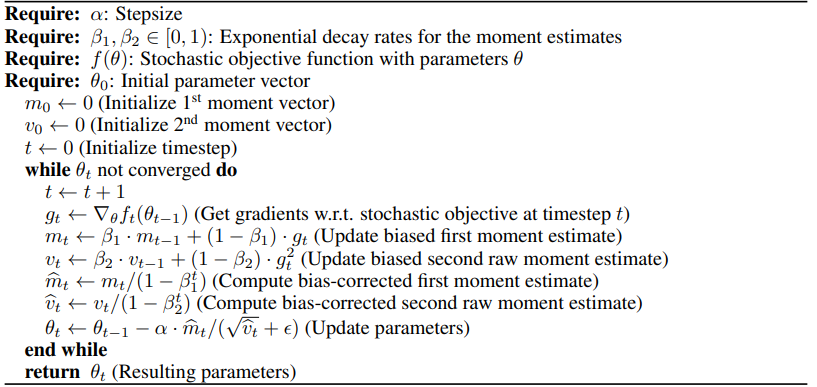
\includegraphics[scale=0.4]{pseudocode.png}
\end{center}









\newpage
\section{Results}

We evaluated four optimizers in different settings on a neural network with two convolution layers and two fully connected layers with relu as the non-linear function, and trained it to recognize hand written digits from 0 to 9 (known as the MNIST dataset). We compared ADAM, SGD, RMSprop and Adadelta, with different hyperparameters.\\

In the following figure we can see the results of 3 experiments with learning rates of 0.1, 0.01, 0.0001. In all of them the batch size is 512 and all lines were smoothed for better visual evaluation.

\begin{figure}
     \centering
     \begin{subfigure}[b]{0.3\textwidth}
         \centering
         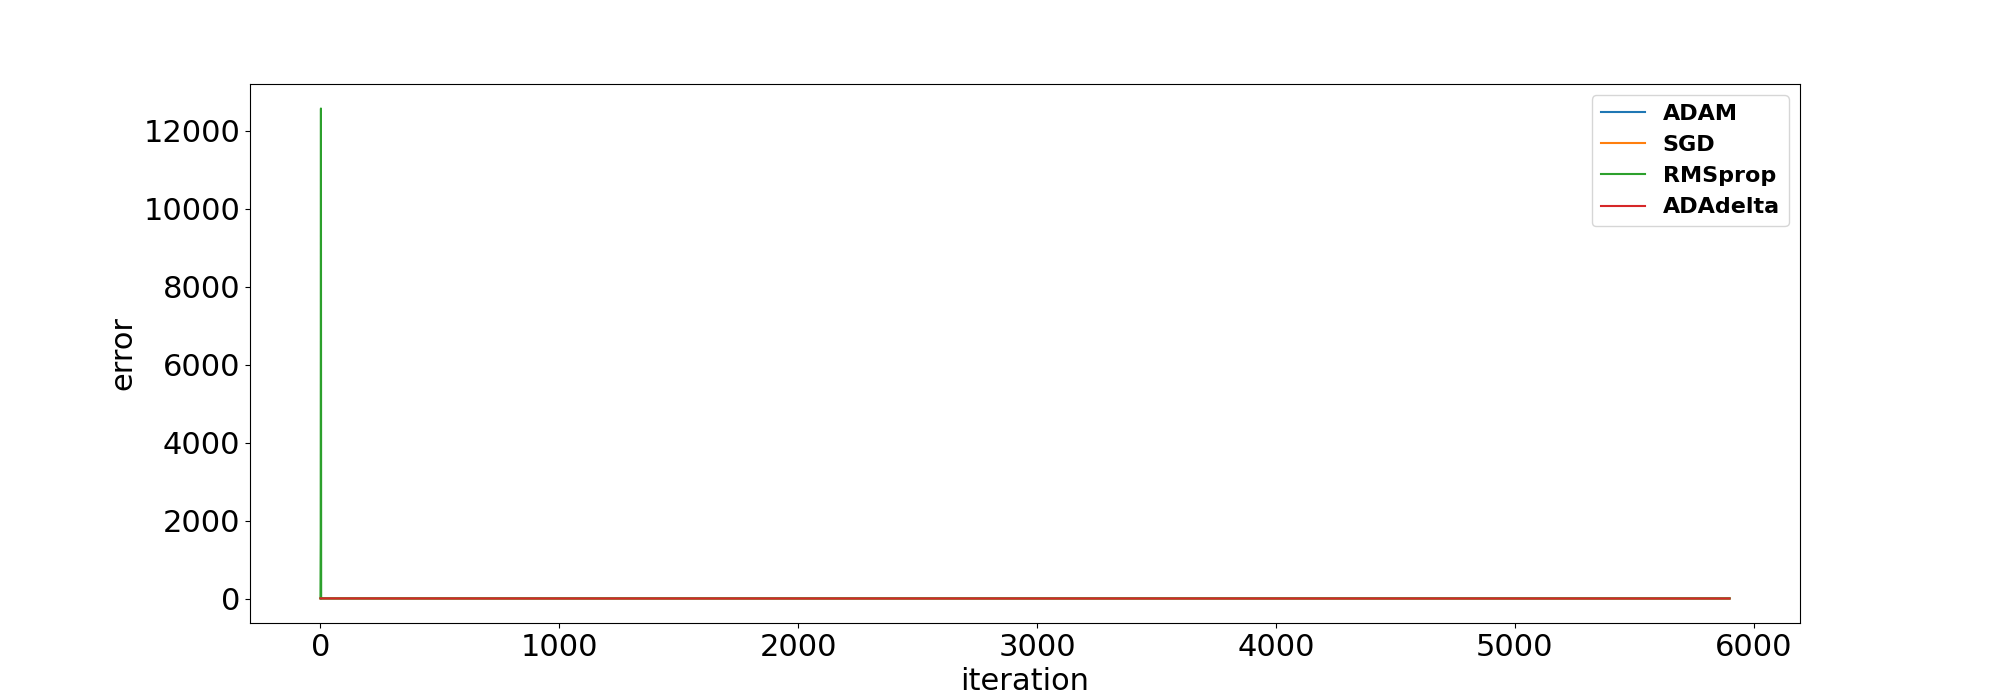
\includegraphics[width=1.5\textwidth]{train_lr=0.1.png}
         \caption{train, $\eta = 0.1$}
         \label{fig: $\eta = 0.1$}
     \end{subfigure}
     \hfill
     \begin{subfigure}[b]{0.3\textwidth}
         \centering
         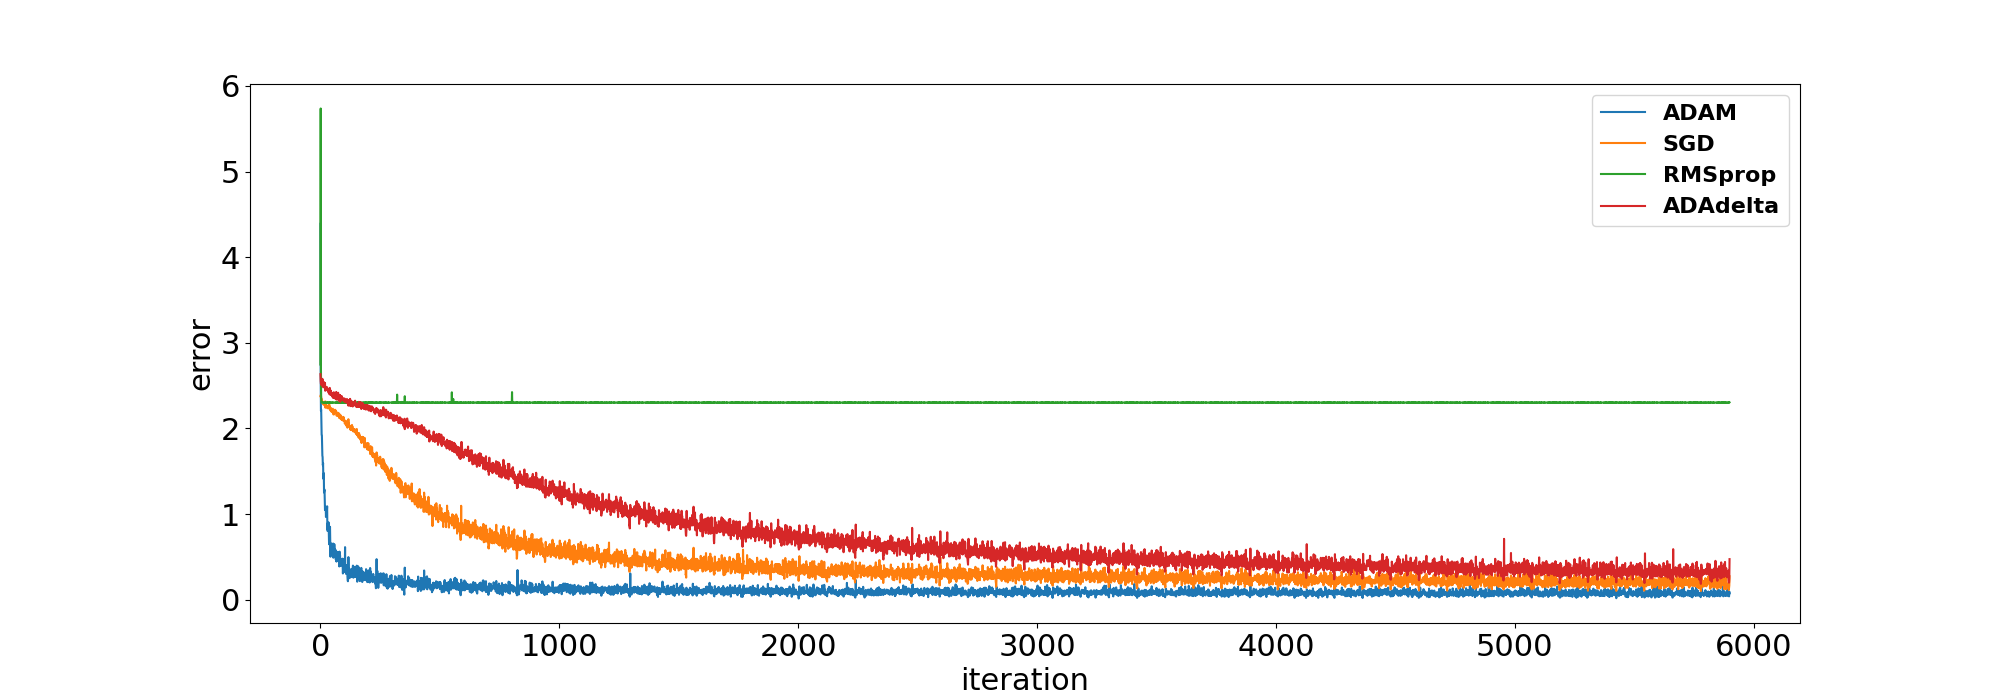
\includegraphics[width=1.5\textwidth]{train_lr=0.01.png}
         \caption{train, $\eta = 0.01$}
         \label{fig:$\eta = 0.01$}
     \end{subfigure}
     \hfill
     \begin{subfigure}[b]{0.3\textwidth}
         \centering
         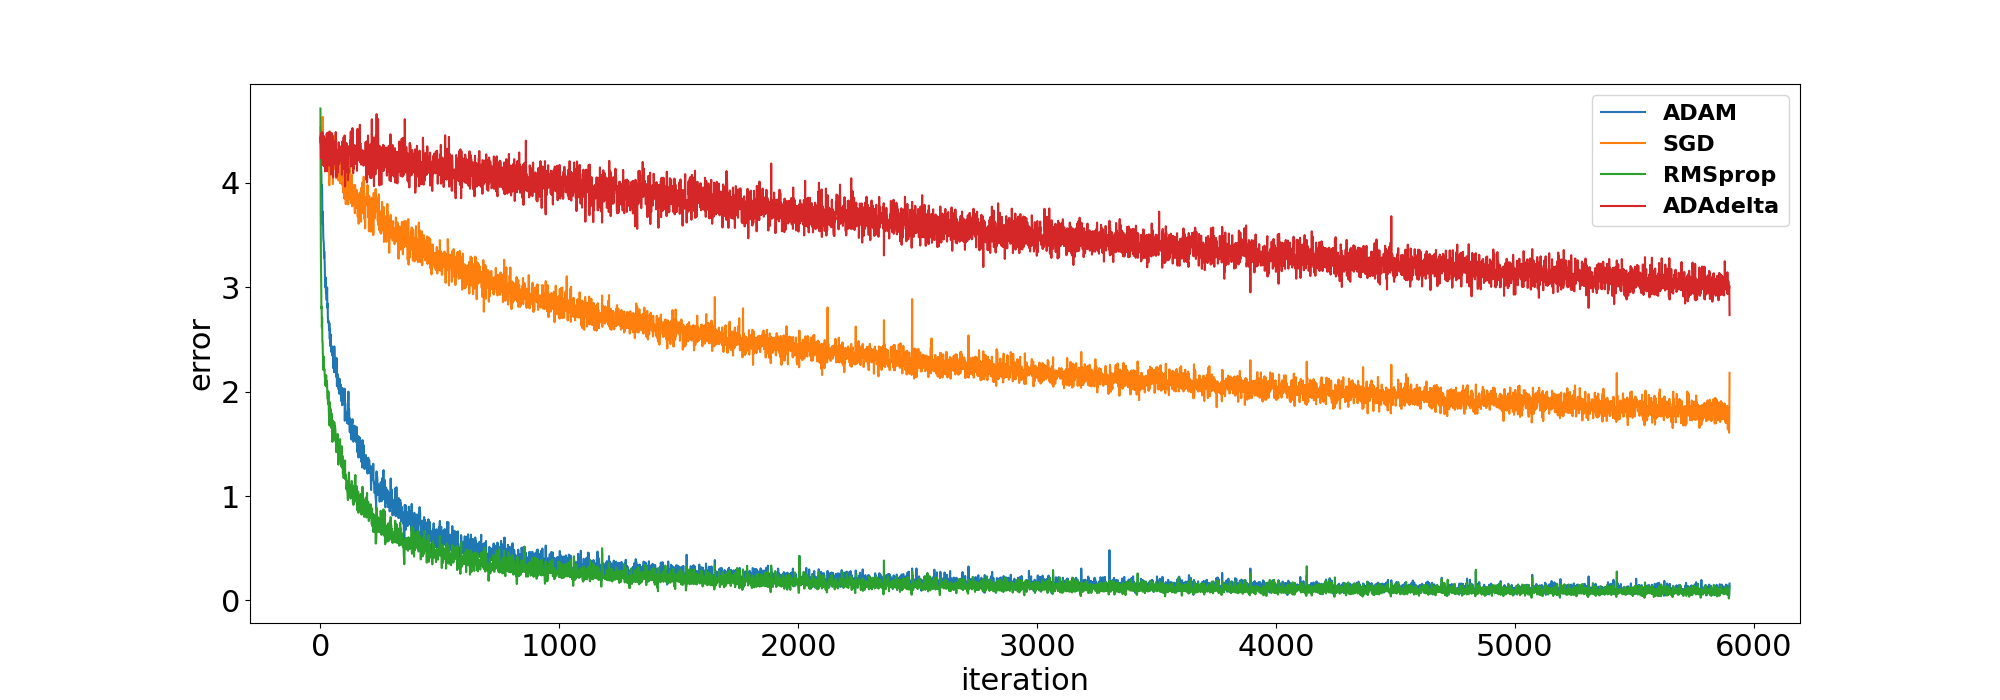
\includegraphics[width=1.5\textwidth]{train_lr=0.0001.png}
         \caption{train, $\eta = 0.0001$}
         \label{fig:$\eta = 0.0001$}
     \end{subfigure}
     \hfill
     \begin{subfigure}[b]{0.3\textwidth}
         \centering
         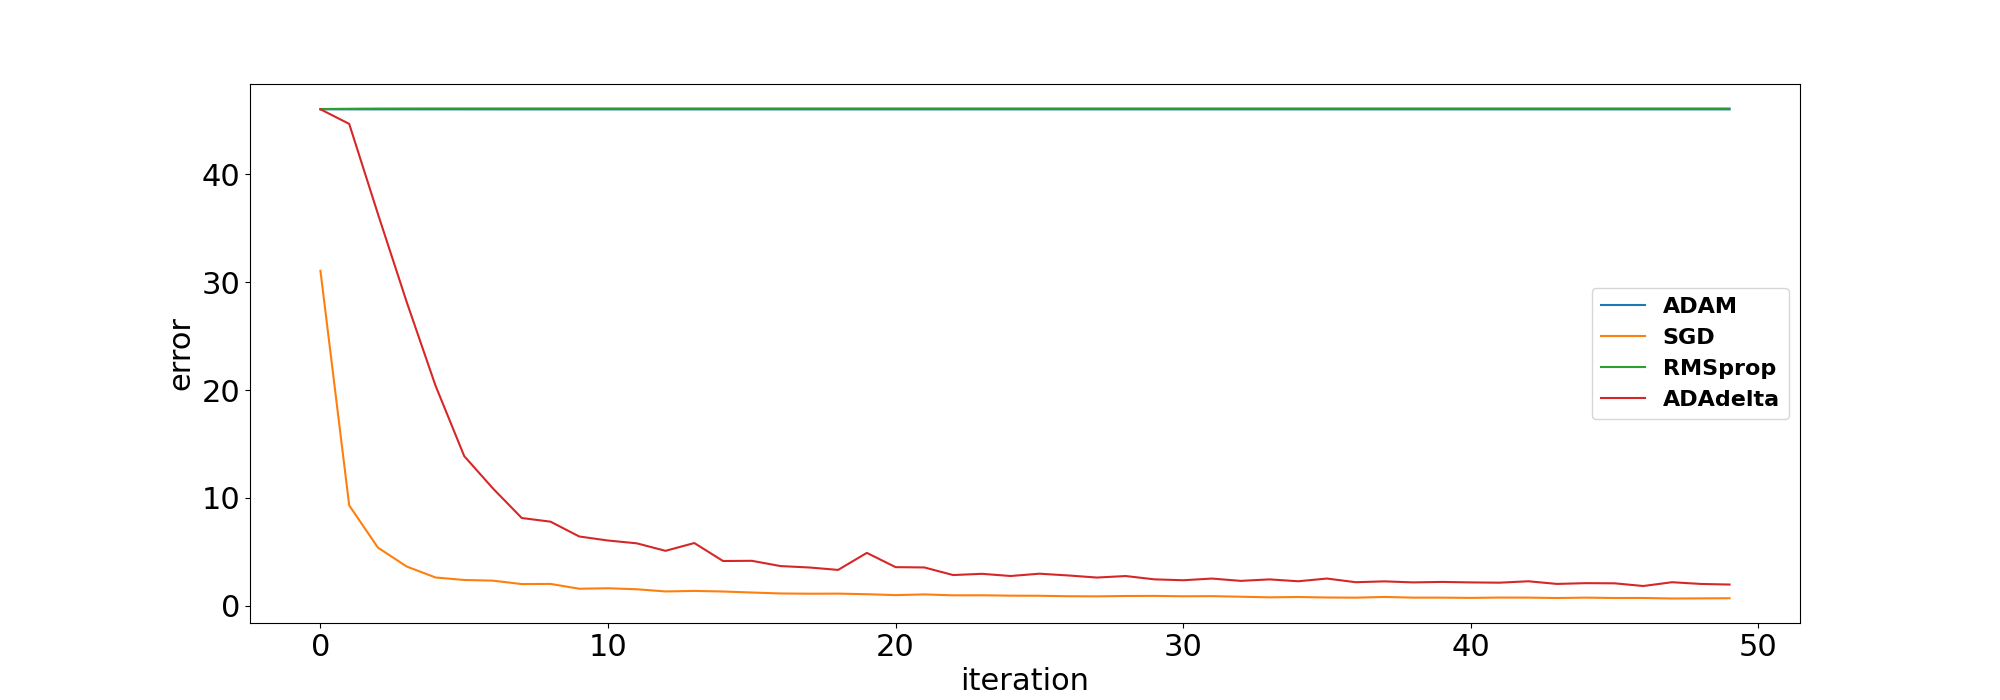
\includegraphics[width=1.5\textwidth]{test_lr=0.1.png}
         \caption{train, $\eta = 0.1$}
         \label{fig:$\eta = 0.1$}
     \hfill
     \end{subfigure}
     \begin{subfigure}[b]{0.3\textwidth}
         \centering
         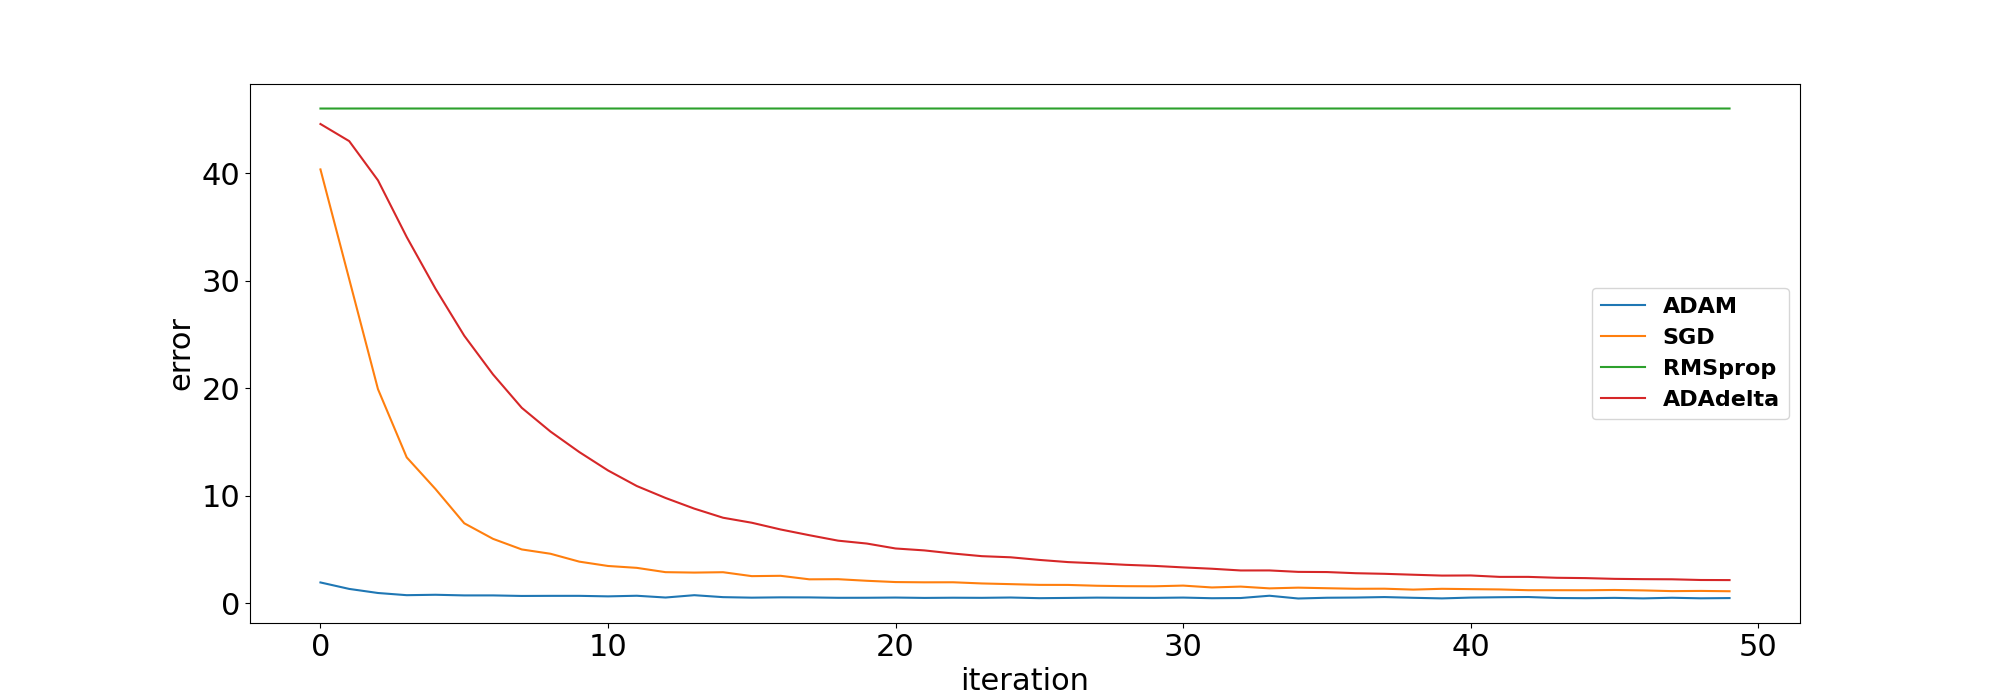
\includegraphics[width=1.5\textwidth]{test_lr=0.01.png}
         \caption{test, $\eta = 0.01$}
         \label{fig:$\eta = 0.01$}
     \end{subfigure}
     \hfill
     \begin{subfigure}[b]{0.3\textwidth}
         \centering
         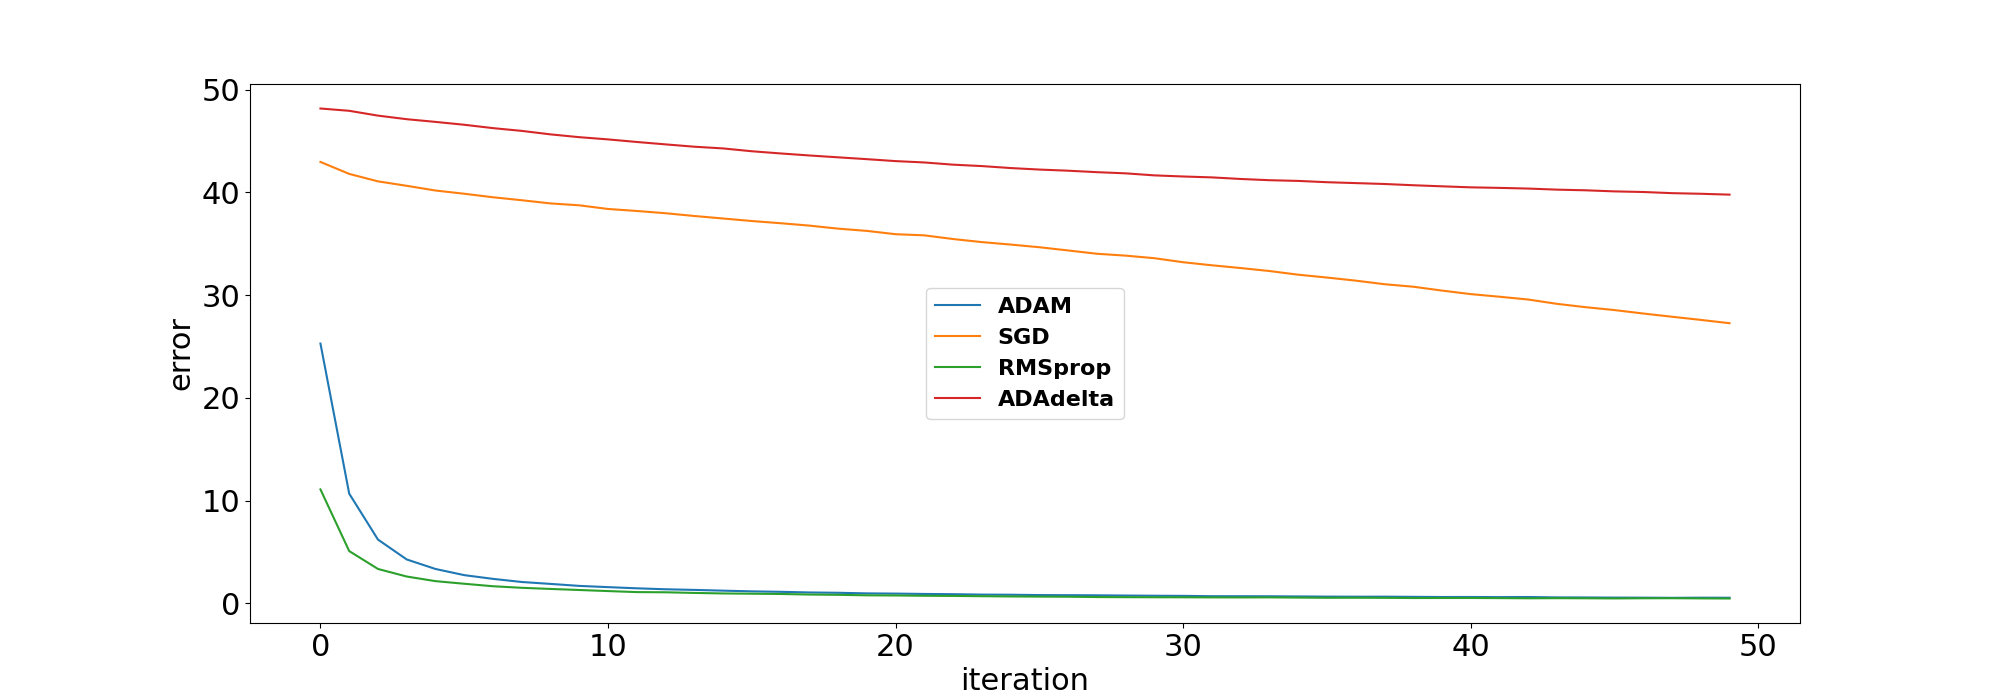
\includegraphics[width=1.5\textwidth]{test_lr=0.0001.png}
         \caption{test, $\eta = 0.0001$}
         \label{fig:$\eta = 0.0001$}
     \end{subfigure}
        \caption{Three simple graphs}
        \label{fig: loss as function of iterations, on train set and test set with different learning rate}
\end{figure}


In figure 1(a) We can see that it converge to a slightly smaller loss, but it took almost twice as long to get this value. We also can see that SGD suffer greatly from decreasing the learning rate since has a bad convergence rate. Adadelta also suffer and provide the worst convergence rate. If we continue to iterate we probably would get a smaller loss value but it would take days. \\

In figure 1(b) We can see Adadelta and SGD has a poor convergance, while RMSprop provide a very good convergance and is very close to the results from ADAM, but still ADAM outperform them all.\\

In figure 1(c), with the lowest learning rate, We can see SGD and Adadelta converge to a similar value as ADAM, but still ADAM provide a better convergence rate. We also can see that RMSprop does not learn properly and got stuck on high loss value, this is due to the lack of momentum term in RMSprop, that got it stuck at a high minima or saddle point, in contrast to ADAM and Adadelta who have a momentum term.\\

*
*
* add explanations for test graphs 
*
*
*\\

\section*{Add here the results where Adam is not good}

\section{Discussions}
In \cite{vaswani2019painless}, the authors argue that althogh ADAM provide extremely good results on deep learning optimization i.e. trying to optimize a loss surface, it provide extremey poor results on other optimization problems.
The key difference between deep learning model optimization, is the shear number of parameters to optimize (several millions), and that derivatives of the error function are ususally ill conditioned \cite{li2017visualizing}, thus the error surface has many saddle points, thus from one hand convex optimization is not feasible in this cases, and in the other hand second order optimization is not feasible dus to the high dimensionality of parameters, which will require $O(n^2)$ in memory. This is where ADAM shines, it doesn't require more than calculating the gradients themselves, like SGD, but its momentum allows it to overcome local minima and saddle points, with its ability to properly tune the learning rate to different parameters.














\section{More about Other Algorithms}
\textbf{Batch Gradient Descent} As mentioned in section 1, BGD passes through the whole dataset in batches, and store all the gradients in its path, lastly it performs the update step with fixed learning rate $\theta:=\theta-\eta \nabla_\theta L(\theta)$. \\



\textbf{Stochastic Gradient Descent} As we mentioned above vanilla SGD, is just apllying to each parameter the gradient of the error, with some learning rate, $\theta:=\theta-\frac{\eta}{n}\sum_{i=1}^{n}\nabla_\theta L_i(\theta;x_i,y_i)$. It is worth mentioning that almost all stochastic approach (including ADAM) have a notable quality that make them perform better on non-convex problems, the stochasity of the formulation makes it easy for them to stay away from local minimas, this also make them possibly miss the global minima or not converge exactly to it, especially in the case of SGD with a fixed learning rate. In the vanilla setup the error of convergence to a global minima in a covex setting of SGD is in the order of the learning rate, but if we add to vanilla SGD a learning rate schedule as suggested in \cite{darken1992learning} we can achieve the same optimal solution as in BGD.\\
The stochastic optimization process with Stochastic Gradient Descent (SGD), $D$, $f(x)$, $\hat{f}_{\theta}(x)$ and $\eta$  goes as follows:
\begin{enumerate} 
    \item Randomly sample a batch $b$ of samples from the dataset $b \in D$.
    \item Get the estimated function $\hat{f}_{\theta}(b)$, by running $b$ through the model.
    \item Evaluate the objective function $L(\theta) = \frac{1}{n} \sum_{i=1}^{n} L_i(\theta)$ using $f(\theta)$ and $\hat{f}_{\theta}(b)$.
    \item Update the parameters $theta$ as follows: $\theta:=\theta-\frac{\eta}{n}\sum_{i=1}^{n}\nabla L_i(\theta)$
\end{enumerate}



\textbf{Mini batch Gradient Descent} is the combination of BGD and SGD, we do itterate over the all dataset in random batches, but update the parameters each batch, thus acheiving convergence much faster and still have the property of stochasity.
The key withdraw of all variants of gradient descent comparimg to ADAM (or other adaptive methods) is they use a learning rate which the user needs to wisely choose and is the same for all parameters, another key chalenge for those algorithms is saddle points, they do not perform well in smooth plateaus, which are common in deep learning \cite{dauphin2014identifying}.\\
As we mentioned earlier ADAM stands for adaptive moment estimation, the term adaptive refers to the property that ADAM calculates adaptive learning rates for each parameter, in contrast to SGD, in which the learning rate is fixed to all the parameters. This property is similar to other adaptive methods, such as Adadelta, Adagrad and RMSprop.\\


\textbf{Adagrad} is a gradient-based optimization algorithm that adapts the learning rate to the parameters, performing smaller updates for parameters associated with frequently occurring features, and larger updates (i.e. high learning rates) for parameters associated with infrequent features.\\


Let's denote $g_{t, i} = \nabla_\theta J( \theta_{t, i} )$, which is the partial derivative of the objective function w.r.t its parameters $\theta_i$, we calculate a diagonal matrix $G_t$, where each element is $G=\sum_{i=1}^{N} g_i g_i^T$, where N is the number of itterations, thus the update rule is $\theta_{t+1, i} = \theta_{t, i} - \dfrac{\eta}{\sqrt{G_{t, ii}} + \epsilon} \cdot g_{t, i}$
This method is well suited for sparse data because of its adaptivity to occurence of features.
\\

\textbf{Adadelta} 
\\

\textbf{RMSprop} was also introduced due to the shortcomings of Adagrad in regard to its quick decreasing of learning rate, it calculates the running average of past squared gradients $E[g^2]_t = \gamma E[g^2]_{t-1} + (1 - \gamma) g^2_t$, and the update rule is $\theta_{t+1} = \theta_{t} - \dfrac{\eta}{\sqrt{E[g^2]_t} + \epsilon} g_{t}$, we can see it is similar to the variance term in ADAM except the running average in RMSprop is only over the previous average of square gradients and ADAM is exponentially moving.
The other property of ADAM is moment estimation, ADAM calculates past gradient averages, similarly to momentum methods and in fact can be seen as a combination of a momentum method that does not calculate the variance and RMSprop that do not calculate the average, and lacks the term regarding the first moment averaging.\\

\textbf{AMSGrad} In \cite{reddi2019convergence} the authors argue that ADAM do not converge well to an optimal solution for convex problems, due to the exponential moving avergae of the gradients, which result in forgettness of long-term memory of past gradients. Therefor suggest an alternative AMSGrad which is a corrected version of ADAM, which replaces $\hat{v}_t$ to be $\hat{v}_t = \max(\hat{v}_{t-1}, v_t)$, all in all the authors get a similar algorithm to ADAM, but found that the de-biasing can be avoided, thus getting:
\begin{align} 
    \begin{split} 
    m_t &= \beta_1 m_{t-1} + (1 - \beta_1) g_t \\ 
    v_t &= \beta_2 v_{t-1} + (1 - \beta_2) g_t^2\\ 
    \hat{v}_t &= \text{max}(\hat{v}_{t-1}, v_t) \\ 
    \theta_{t+1} &= \theta_{t} - \dfrac{\eta}{\sqrt{\hat{v}_t} + \epsilon} m_t 
    \end{split} 
\end{align}
    
where $v_t$ is the regular moving average for the variance
this fixes the forgetness of ADAM and was shown to perform better on convex problems than ADAM, and we get an update rule similar to ADAM but never get an increasing step-size (which is to blame for its inability to converge).\\
Where ADAM shines is actually in non-convex error surface such as deep learning models (where it is widley used), and in \cite{chen2018convergence}, the authors even provided an upper bound for convergence rate under some mild conditions, but the authors showed that in some cases of deep learning problems AMSgrad outperforms ADAM.\\



\section{Miscellanea}

In \cite{vaswani2019painless}, the authors argue that althogh ADAM provide extremely good results on deep learning optimization i.e. trying to optimize a loss surface, it provide extremey poor results on other optimization problems.
The key difference between deep learning model optimization, is the shear number of parameters to optimize (several millions), and that derivatives of the error function are ususally ill conditioned \cite{li2017visualizing}, thus the error surface has many saddle points, thus from one hand convex optimization is not feasible in this cases, and in the other hand second order optimization is not feasible dus to the high dimensionality of parameters, which will require $O(n^2)$ in memory. This is where ADAM shines, it doesn't require more than calculating the gradients themselves, like SGD, but its momentum allows it to overcome local minima and saddle points, with its ability to properly tune the learning rate to different parameters.


\bibliography{proj}
\bibliographystyle{plain}

\section{The Code}
\begin{lstlisting}[language=python]

def loss_function(x):
    return x ** 3 - 3 * x ** 2 + 4 * x


def grad_function(x):
    return 3 * x ** 2 - 6 * x


def check_convergence(theta0, theta1):
    return all(theta0 == theta1)


theta = np.random.rand(5)
num_iter = 10
converged = False
adam = my_adam.adam_optimizer(theta)
d_theta = np.zeros_like(theta)
old_theta = np.zeros_like(theta)
loss_values = []

while not converged:
    for i, theta_i in enumerate(theta):
        d_theta[i] = grad_function(theta_i)
        old_theta = theta_i
    theta = adam.step(num_iter, theta, d_theta)
    loss_values.append(loss_function(theta_i))
    if check_convergence(theta, old_theta):
        print('number of iterations until ADAM converged: ' + str(num_iter))
        break
    else:
        print('iteration number ' + str(num_iter) + ' : weight = ' + str(theta))
        num_iter += 1

import numpy as np


class adam_optimizer:
    def __init__(self, theta, step_size=0.01, beta1=0.9, beta2=0.999, epsilon=1e-8):
        self.mean_d_theta = np.zeros_like(theta)
        self.u_variance_d_theta = np.zeros_like(theta)
        self.beta1 = beta1  # beta1 is the exponential decay of the rate for
                                         the first moment estimates
        self.beta2 = beta2  # beta2 is the exponential decay rate for
                                         the second-moment estimates
        self.epsilon = epsilon  # prevent zero-division
        self.step_size = step_size

    def step(self, num_iter, theta, d_theta):
        mean_d_theta_corr = np.zeros_like(theta)
        u_variance_d_theta_corr = np.zeros_like(theta)
        for i, theta_i in enumerate(theta):
            self.mean_d_theta[i] = self.beta1 * self.mean_d_theta[i]
                    + (1 - self.beta1) * d_theta[i]
            self.u_variance_d_theta[i] = self.beta2 * self.u_variance_d_theta[i] 
                    + (1 - self.beta2) * (d_theta[i] ** 2)

            # the bias correction step
            mean_d_theta_corr[i] = self.mean_d_theta[i] 
                    / (1 - self.beta1 ** num_iter)
            u_variance_d_theta_corr[i] = self.u_variance_d_theta[i] 
                    / (1 - self.beta2 ** num_iter)

            # update weights and biases
            theta[i] = theta[i] - self.step_size * (mean_d_theta_corr[i] 
                    / (np.sqrt(u_variance_d_theta_corr[i])+ self.epsilon))
        return theta

\end{lstlisting}

\end{document}

